\section{Technische Detailspezifikation}
\subsection{Innere Struktur}
\subsubsection{Struktur des Systemdesigns}
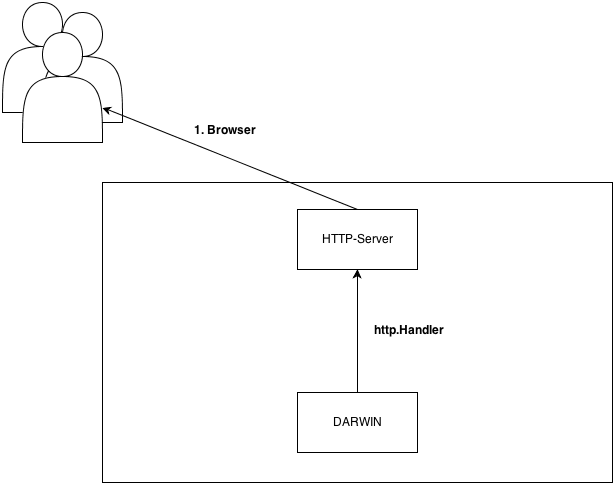
\includegraphics[width=\linewidth]{simplearch.png}
\subsubsection{Beschreibung der Elemente}
Die Architektur von darwin besteht aus 3 Hauptkomponenten.
\subsubsection{Die Spieler}
DARWIN ist ein Multiplayerspiel für bis zu 4 Spieler. Die Spieler können sich via
Netzwerk auf den Server verbinden. Zum Spielen wir ein Browser verwendet.
\subsubsection{Der HTTP-Server}
DARWIN selbst implementiert einen HTTP-Server aus den Standard-Packages von \bold{go}.
Der HTTP-Server wird für das Hosten der zum Spielen benötigten HTML5-Seiten und
Javascripts verwendet.
\subsubsection{DARWIN (Das Spiel)}
Das Spiel selbst implementiert die allgemeine Spielstruktur welche aus einem Websocket-Server und dem Spiel an sich besteht. Der Websocket-Server implementiert das http.Handler Interface um sich beim HTTP-Server zu registrieren.
\subsection{Schnittstellendefinitionen}
Es werden hauptsächlich zwei Interfaces verwendet.
\subsubsection{1. Browser}
Der Browser stellt die Schnittstelle der Spieler zum Server dar. Diese wurde
mithilfe der Technologien HTML5 und Javascript realisiert.
\subsubsection{http.Handler}
Die http.Handler Schnittstelle wird dazu verwendet eine Methode beim HTTP-Server zu registrieren damit diese per URL-Aufruf ausgeführt wird.
\subsection{Sicherheit}
\subsection{Anforderungszuordnung}

